%!TEX root = ../../prace.tex

\section{Herní menu - ukládání, nahrávání}

V průběhu rozehrané hry je možné použít \textbf{Rychlé uložení / načtení}, nebo si hru uložit z~herní nabídky.

Pro uložení hry je možné vytvořit nový save nebo přepsat stávající, pokud nějaký existuje. Uložené hry je též možné mazat.

\begin{figure}[!ht]\centering
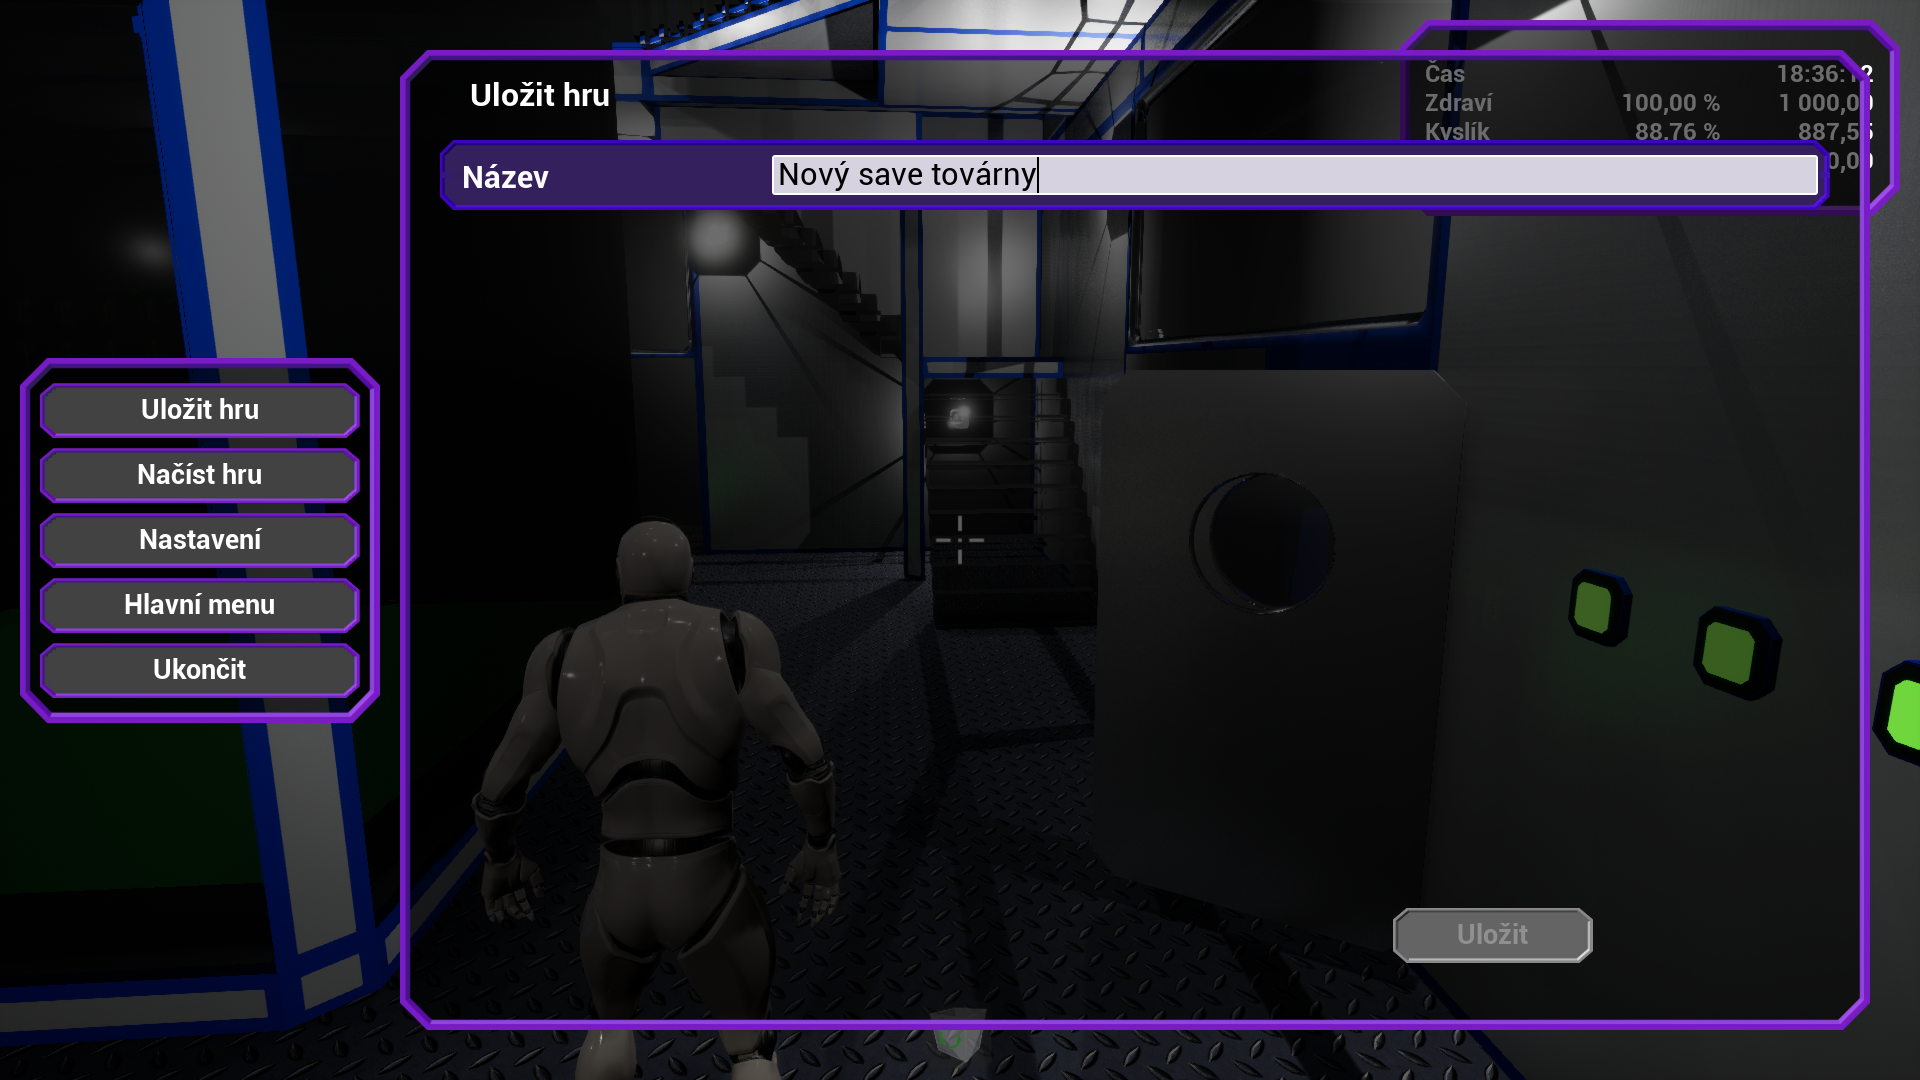
\includegraphics[ width=140mm]{../img/user/save/0newSave}

\caption{Ukládání - Nový save}
\label{fig:user_save_0newSave}

\end{figure}
\FloatBarrier

Pokud bylo uložení úspěšné, hráči se zobrazí následující hláška:

\begin{figure}[!ht]\centering
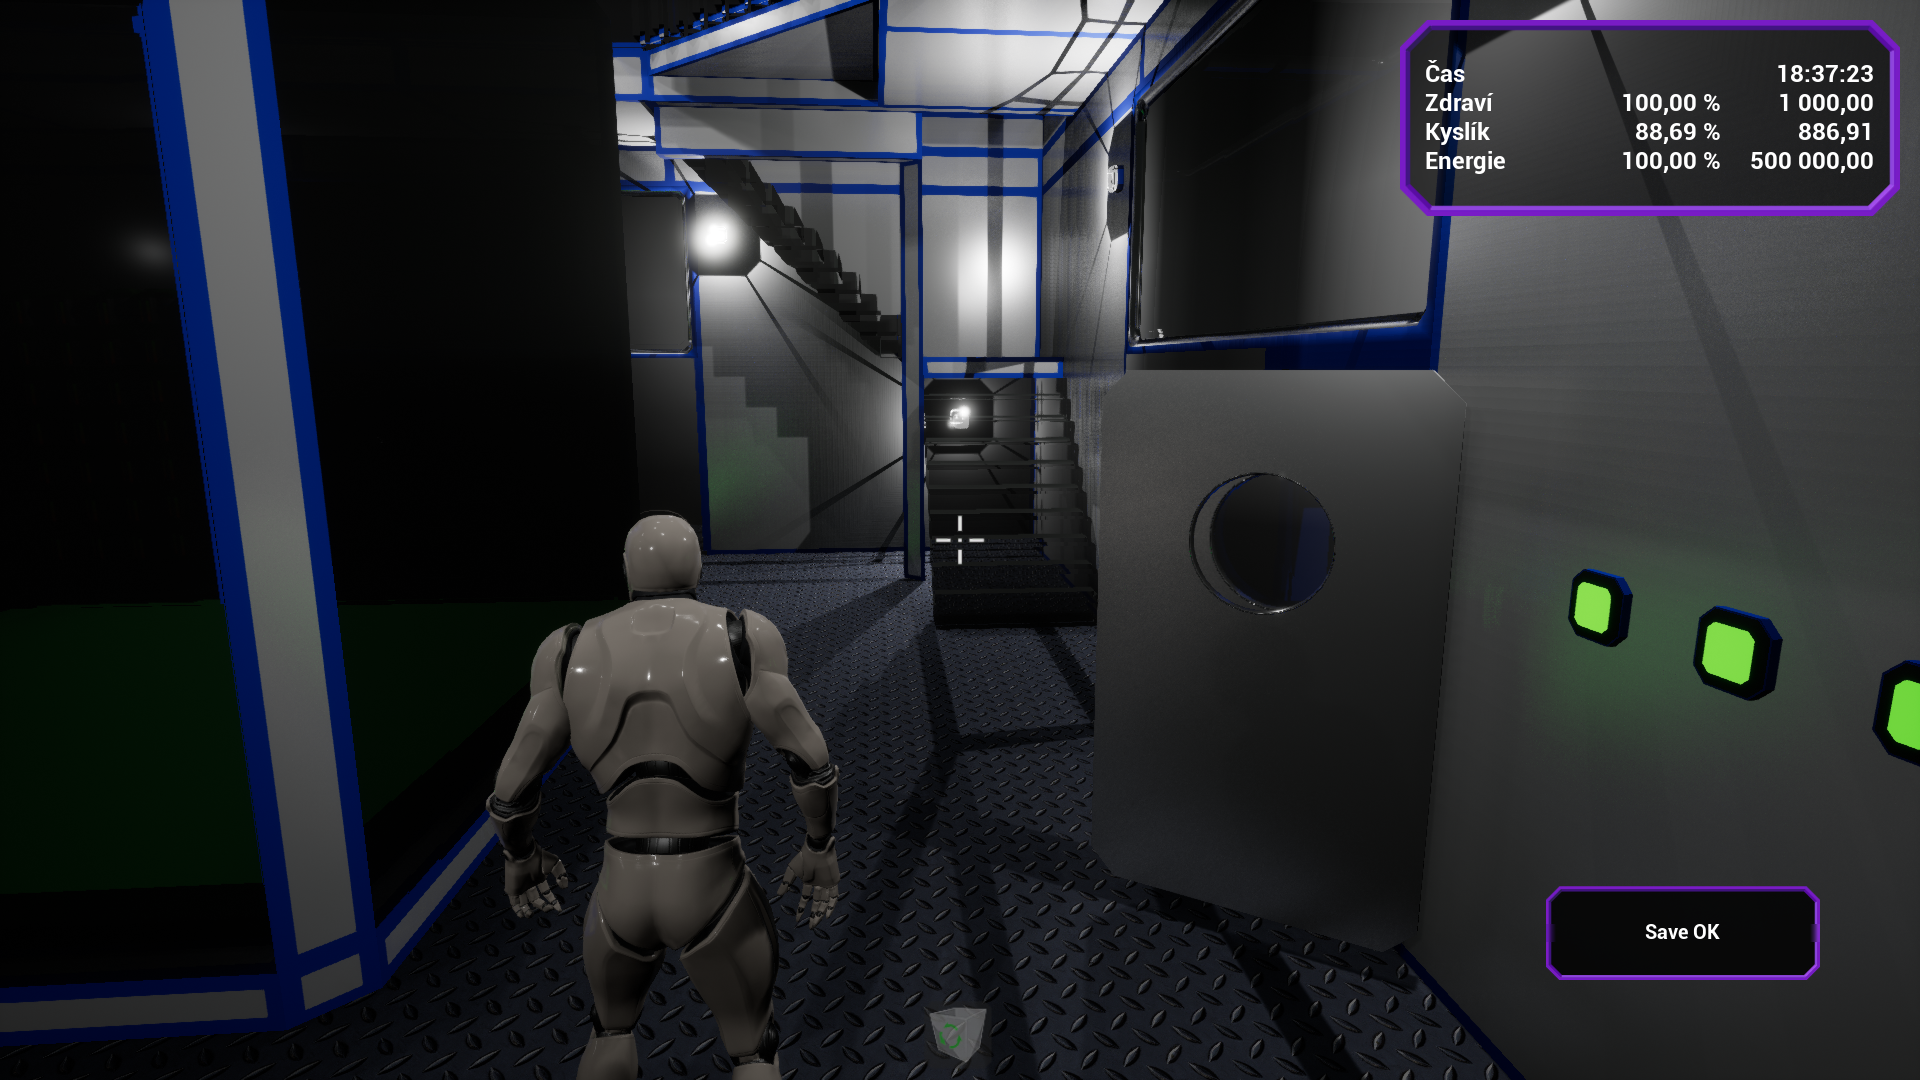
\includegraphics[ width=140mm]{../img/user/save/1afterSave}

\caption{Ukládání - po uložení}
\label{fig:user_save_1afterSave}

\end{figure}
\FloatBarrier

Nahrávat je možné ze všech uložených pozic, včetně rychlého uložení. Opět je zde možné vybraný save smazat.

\begin{figure}[!ht]\centering
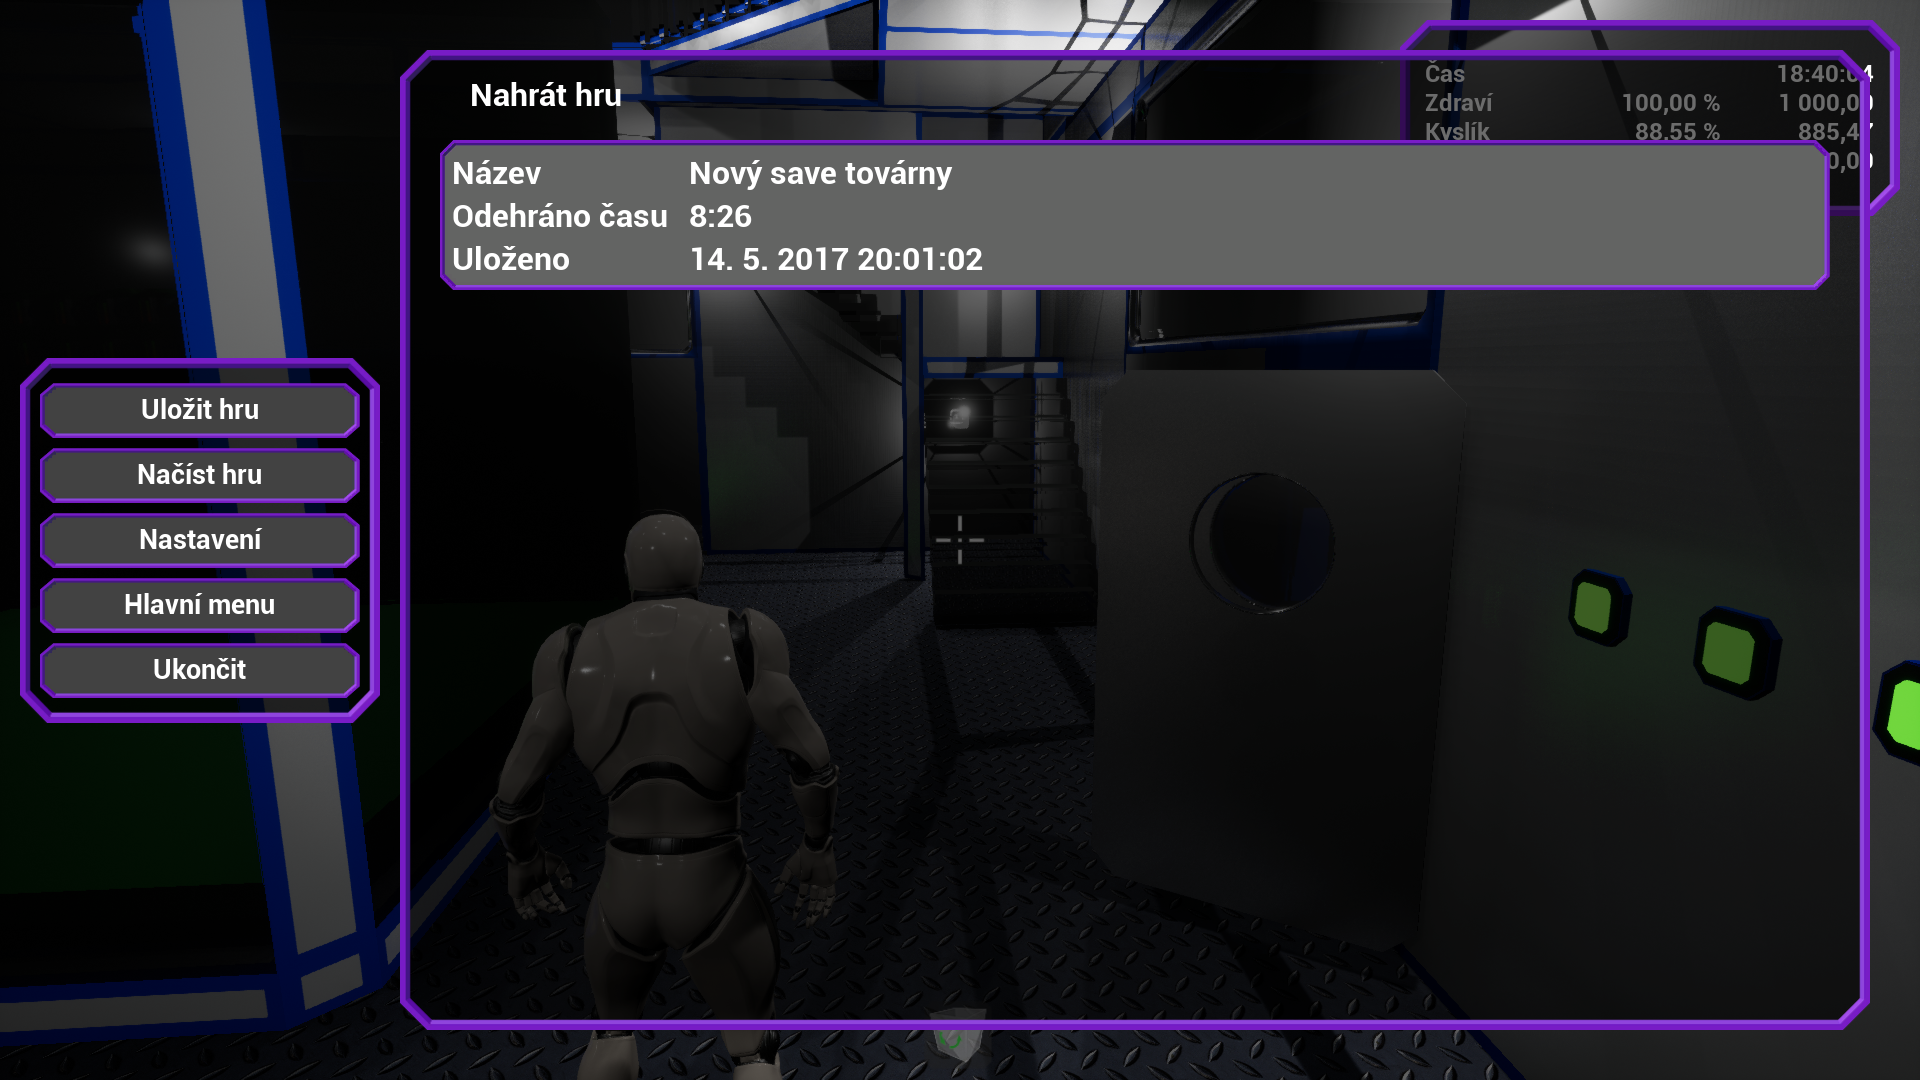
\includegraphics[ width=140mm]{../img/user/save/2load}

\caption{Ukládání - nahrát hru}
\label{fig:user_save_2load}

\end{figure}
\FloatBarrier

Pokud má hráč rozehranou hru, je pro jistotu vyžadováno potvrzení.

\begin{figure}[!ht]\centering
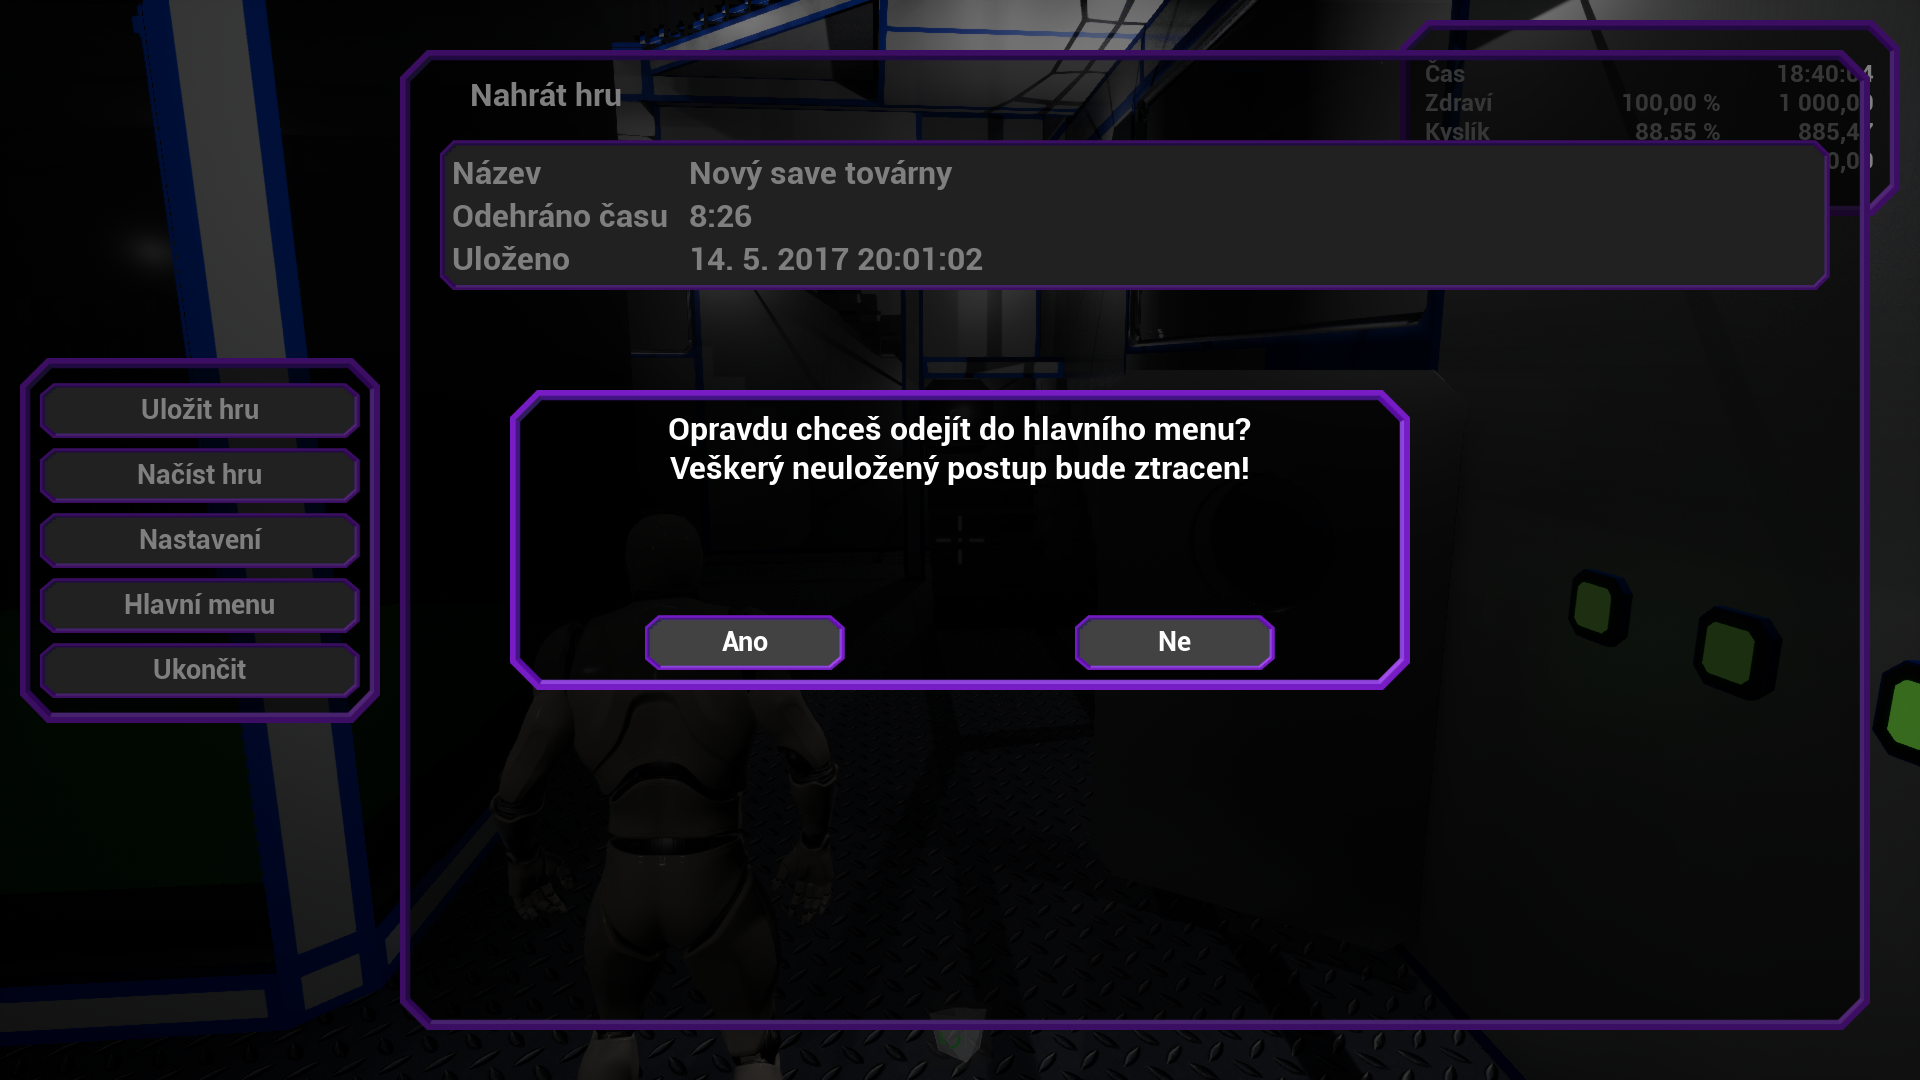
\includegraphics[ width=140mm]{../img/user/save/3loadClicked}

\caption{Ukládání - potvrzení nahrání hry}
\label{fig:user_save_3loadClicked}

\end{figure}

\FloatBarrier